\appendixchapter{Engineering block diagram}{i}
\label{appendixA}

\autoref{fig:engineeringBlockDiagram} shows the relationship of the recommended end-user naming provided in \autoref{fig:schematic} to the engineering-centric block diagram that may be familiar to adopters of pre-release ACES. As noted above, the acronyms such as IDT, LMT, RRT, and ODT are oriented towards color scientists and post-production engineers and are discouraged from use in products.

\begin{figure}[htbp]
\begin{center}
    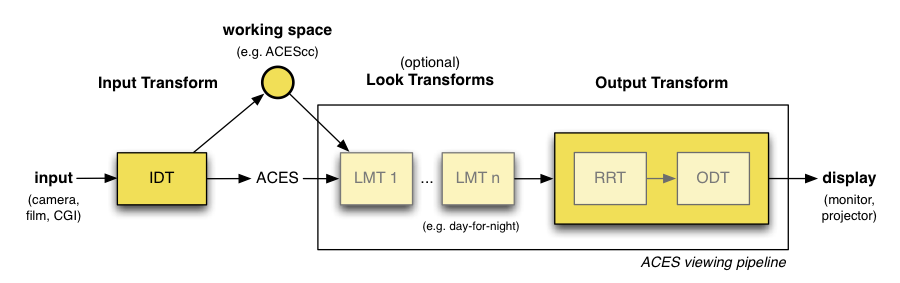
\includegraphics[width=\textwidth]{engineeringBlockDiagram.png}
\caption{End-user naming shown in relation to the engineering-centric block diagram}
\label{fig:engineeringBlockDiagram}
\end{center}
\end{figure}

\textbf{Engineering-centric acronyms}

IDT (Input Device Transform) -- Converts colors from an input device (such as a digital cinema camera or film scanner) into ACES2065-1 color space. Please refer to Academy P-2013-001.

LMT (Look Modification Transform) -- Imparts an image-wide creative ‘look’ to the appearance of ACES images. The input and output color space is ACES2065-1. Please refer to Academy TB-2014-010.

RRT (Reference Rendering Transform) -- Converts the scene-referred ACES2065-1 colors into colorimetry for an idealized cinema projector with no dynamic range or gamut limitations.

ODT (Output Device Transform) -- Takes the output of the RRT and applies additional dynamic range compression and gamut adjustment followed by encoding of the desired colorimetry for a specific display device calibration aim.

\note{For the reasons discussed earlier in this document, usage of these terms in product user interfaces is deprecated.}

